\label{strings}
\begin{chapterbox}
\vspace{-60pt}
\chapter{String Theory}
\vspace{-30pt}
\centering\normalsize\textit{Lent Term 2018 - Professor P. Townsend}
\end{chapterbox}
\vspace{20pt}
%\begin{multicols*}{2}
\minitoc
\newpage
\section{Prehistory/History}
Start with a prehistory from around $1920$, well before the current formulation of the subject. Consider some string with a tension $T$, and mass density $\rho$, then the velocity of small amplitude waves is;
\begin{equation}
v = \sqrt{\frac{T}{\rho}}
\end{equation}
Classically this velocity could increase without bound, however relativity enforces $v \leq c$, so we have the bound;
\begin{equation}
T \leq \rho c^2
\end{equation}
For an ordinary string, $T \ll \rho c^2$, representing the non-relativistic limit. In the ultra-relativistic\index{ultra-relativistic} limit however $T = \rho c^2$. This is the string of string theory and cosmic strings\footnote{It is also Ehrenfest's toy model for Electromagnetism which was quantised by Jordan in 1926 to give the first true quantum field theory}\index{cosmic string}. Some consequences of this are;
\begin{enumerate}
\item The system is boost invariant, the displacement still travels at speed $c$
\item The string cannot carry longitudinal modes
\end{enumerate}
We also know that since the tension is $-P$, where $P$ is the pressure, in the ultra-relativistic limit, the material must have a Lorentz invariant\index{Lorentz invariant} energy-momentum tensor\index{tensor!energy-momentum};
\begin{equation}
T_{\mu \nu} = \rho \etamn{_}
\end{equation}
Moving on to the 1960s, Hadron resonances\index{hadron resonances} appeared to lie on \emph{Regge trajectories}\index{Regge trajectories};
\begin{mygraphic}{strings/regge}{0.5}{Measurements suggested the particles (mesons) lay on trajectories $M^2 = \tfrac{J - \alpha_0}{\alpha\pr}$, where $J$ is the spin of the particle.}{regge}\end{mygraphic}
However, if this were to continue indefinitely, there are problems at high energies. These can be avoided if the resonances (in the s-channel\index{s-channel}) are also exchanged (in the t-channel\index{t-channel}). 
\begin{mygraphic}{strings/resonance}{0.5}{The resonances in the s-channel (left) should be the same as in the t-channel. In other words, the same particle should be exchanged in both processes.}{resonances}\end{mygraphic}
In 1969, Veneziano wrote down a formula for the amplitude $\mathcal{A}$ for processes such as that shown in \autoref{fig:resonances}. In 1970, this was interpreted as an open string. In terms of mesons, you can think of this as a quark-antiquark\index{quark}\index{quark!antiquark}. This gave a clear explanation of quark confinement and by considering the strings rotational motion you could generate a mass spectrum. It also introduces a characteristic length scale, the \emph{string length}\index{string length};
\begin{equation}
l_s = \sqrt{\frac{\hbar c}{T}} \sim 10^{-15} \,\,\,\text{m}
\end{equation}
Unfortunately, given this characteristic length scale, you would expect the interior of the interactions such as those in \autoref{fig:resonances} to be soft. But this doesn't agree with experiments; we see quarks etc. So the string theory of hadrons was abandoned, replaced by a string theory of quantum gravity. This entailed considering closed strings and taking the string length to be of order Planck length\index{Planck length};
\begin{equation}
l_s = \sqrt{\frac{\hbar G}{c^4}} \sim 10^{-35} \,\,\,\text{m}
\end{equation}
This had it's own issues however, the ground state was found to be a tachyon\index{tachyon} with $m^2 < 0$\footnote{This doesn't entail things such as travelling backwards in time etc. Instead, it suggests that the vacuum has an instability; the theory is `sick'.}. More promisingly though, the first excited states are massless and include $J = 2$, which is interpreted as a graviton\index{graviton}. All that remains is to fix the tachyon problem, which is achieved by replacing the string with a superstring\index{superstring}. Supersymmetry\index{supersymmetry} remaining unbroken leads to no tachyons.
\begin{center}
    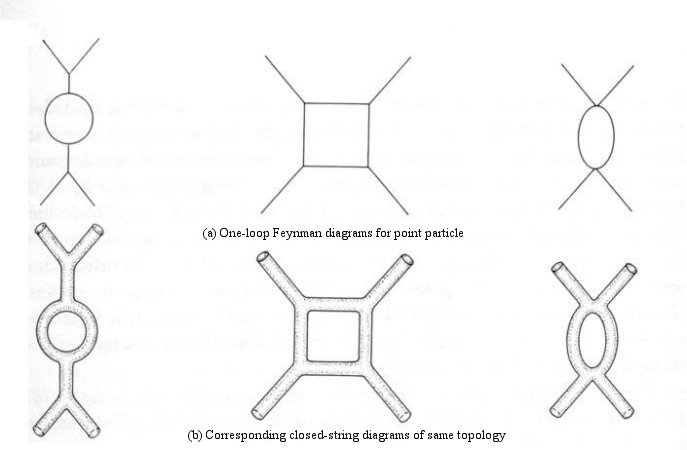
\includegraphics[width=0.7\textwidth]{graphics/strings/stringloop.jpg}
    \captionof{figure}{The correspondence between Feynman diagrams for particles and those for strings. Now there is a non-trivial topology\index{topology} involving holes etc.}
    \label{fig:stringloop}
\end{center}
Returning to amplitudes, we can't use QFT. Instead we need to revert to Feynman's path integral\index{path integral} formulation, mapping particle actions to Feynman diagrams.
\begin{equation}
\int{\mathcal{D}\phi \,\, e^{i S_{\text{particle}}}} \Longrightarrow \int{\mathcal{D}\phi \,\, e^{i S_{\text{string}}}} 
\end{equation}
This is qualitatively different to considering strings as excitations of a string field, which is much harder.
\subsection{The Relativistic Point Particle}
In physical terms, an elementary particle is one without structure, which implies that the classical action should only depend on the geometry of the worldline\index{worldline}, as well as other variables such as spin. The simplest geometric invariant is the proper time on the worldline between two points $A$ and $B$. 
\begin{equation}
I = -mc^2\int_A^B{\ud \tau}
\end{equation}
But $c\ud \tau = \sqrt{-\ud s^2} = \sqrt{-\ud x^\mu \ud x^\nu \etamn{_}}$ with $\etamn{_} = \text{diag}(-1, 1, 1, 1)$, so $c\ud \tau = \sqrt{-\dot{x}^\mu \dot{x}^\nu \etamn{_}} = \sqrt{-\dot{x}^2}\ud t$;
\begin{equation}
\label{eq:earlyaction}
\Rightarrow I[x] = -mc\int_{t_A}^{t_B}{\upd{t}\sqrt{-\dot{x}^2}}
\end{equation}
We'll see later that we are free to choose $x^0 = c\tau$, then;
\begin{equation}
I = -mc^2 \int_{t_A}^{t_B}{\upd{t}\sqrt{\left(x^0\right)^2 - \abs{\dot{\vec x}}^2}} = \int_{t_A}^{t_B}{\upd{t} \set{-mc^2 + \tfrac{1}{2}mv^2 + \mO\left(\tfrac{v^2}{c^2}\right)}}
\end{equation}
\subsubsection{Hamiltonian\index{Hamiltonian} Formalism}
Suppose we take $\mL = -mc^2 + \tfrac{1}{2}mv^2$, then we find happily that $\hamilt = \tfrac{1}{2m}\abs{\vec p}^2 + mc^2$. But suppose instead we start from $\mL = -mc\sqrt{-\dot{x}^2}$, then;
\begin{equation}
p_\mu = \frac{\del \mL}{\del \dot{x}^\mu} = \frac{mc}{\sqrt{-\dot{x}^2}}\etamn{_}\dot{x}^\nu \Rightarrow \dot{x}^\mu p_\mu = -mc \sqrt{-\dot{x}^2}
\end{equation}
But then we find that $\hamilt = 0$...the fact this vanishes is really due to the Hamiltonian generating evolution in a time variable. We can't choose a time parameter uniquely in any Lorentz invariant way, so we shouldn't expect a Hamiltonian. There is another issue though; $p^2 + (mc)^2 = 0$, so the $p^\mu$ aren't independent. As such the phase space isn't even $2n$-dimensional for some $n$. The solution to this, according to Dirac is to relax the identity ($c=1$) $p^2 + m^2 \equiv 0$ and instead impose it as a constraint via a Lagrange multiplier\footnote{We can think of $e$ as a gauge field\index{field!gauge}.} in the action:
\begin{equation}
\label{eq:lmultact}
I(x, p, e) = \int{\upd{t} \dot{x}^\mu p_\mu - \tfrac{1}{2}e(p^2 + m^2)}
\end{equation}
This directly leads to the action in \eqref{eq:earlyaction} via $\tfrac{\delta I}{\delta p} = 0 \iff p^\mu = e^{-1}\dot{x}^\mu$ leading to;
\begin{equation*}
I(x, e) = \frac{1}{2}\int{\upd{t} e^{-1}\dot{x}^2 - m^2 e}
\end{equation*}
Varying with respect to $e$, $\tfrac{\delta I}{\delta e} = 0 \iff e = \tfrac{1}{m}\sqrt{-\dot{x}^2}$ gives the result. Now, we can view \eqref{eq:lmultact} as a field theory in time with $x(t), p(t)$ interpreted as scalar fields\index{field!scalar} and $e(t)$ as a density such that under a transformation $t\pr(t) = t - \xi(t)$;
\begin{equation}
x\pr (t\pr) = x(t), \qquad p\pr(t\pr) = p(t), e\pr (t\pr) \ud t\pr = e(t) \ud t
\end{equation}
Letting $\delta x(t) = x\pr(t) - x(t)$ etc, we find;
\begin{multline}
\delta_\xi x^\mu(t) = \xi(t) \dot{x}^\mu(t) + \mO(\xi^2), \quad \delta_\xi p^\mu(t) = \xi(t)\dot{p}^\mu(t) + \mO(\xi^2), \\ \delta_\xi e(t) = \frac{\ud}{\ud t}\left(e\xi\right)
\end{multline}
Putting this into the Lagrangian; $\mL = \dot{x}^\mu p_\mu - \tfrac{1}{2}e(p^2 + m^2)$, we find that;
\begin{align*}
\mL &\rightarrow  (\dot{x}^\mu + \dot{\xi} \dot{x}^\mu + \xi \ddot{x}^\mu)(p_\mu + \xi \dot{p}_\mu) \\
& \qquad -\tfrac{1}{2}(e + \dot{e}\xi + e\dot{\xi})\left((p^\mu + \xi \dot{p}^\mu)(p_\mu + \xi \dot{p}_\mu) + m^2\right) \\
&= \mL + \dot{\xi}\left(\dot{x}^\mu p_\mu - \tfrac{1}{2}(p^2 + m^2)\right) \\
& \qquad \quad + \xi\left(\ddot{x}^\mu p_\mu + \dot{p}_\mu \dot{x}^\mu -\tfrac{1}{2}\dot{e}(p^2 + m^2) - \tfrac{1}{2}e(\dot{p}^\mu p_\mu + p^\mu \dot{p}_\mu)\right) \\
&= \mL + \frac{\ud}{\ud t}\left(\xi \mL\right)
\end{align*}
So $\mL$ changes by a total derivative and we have a general gauge invariance under one dimensional co-ordinate transformations\footnote{The group is the infinite dimensional $\text{Diff}_1$}, this validates the choice of $x^0 = ct$ we made earlier. The action $I(x, p, e)$ is invariant under a different canonical gauge transformation;
\begin{equation}
\delta_{\alpha} x^\mu = \alpha p^{\mu}, \qquad \delta_\alpha p^\mu = 0, \qquad \delta _\alpha e = \dot{\alpha}
\end{equation}
This leads to;
\begin{align*}
\delta I &= \int{\upd{t} \set{\dot{\alpha}\dot{p}^2 + \alpha \dot{p}^\mu p_\mu - \tfrac{1}{2}\dot{\alpha}(p^2 + m^2)}} \\
&= \int{\upd{t} \set{\tfrac{1}{2}\dot{\alpha}(p^2 - m^2) +  \alpha \dot{p}^\mu p_\mu}} \\
&= \int{\upd{t} \set{\frac{1}{2}\frac{\ud}{\ud t}\left(\alpha(p^2 - m^2)\right)}} \\
&= \left[\frac{1}{2}\frac{\ud}{\ud t}\left(\alpha(p^2 - m^2)\right)\right]^{t_B}_{t_A}
\end{align*}
which vanishes for suitable boundary conditions. So we have a gauge invariance\index{gauge invariance} (which is physically equivalent to the $\text{Diff}_1$ invariance). Now recall the Poisson bracket\index{Poisson bracket} on phase space is given by;
\begin{equation}
\label{eq:PB}
\set{f, g} \overset{\tiny{\text{def}}}{=}\frac{\del f}{\del x^\mu}\frac{\del g}{\del p_\mu} - \frac{\del g}{\del x^\mu}\frac{\del f}{\del p_\mu}
\end{equation}
Then, we see that,
\begin{enumerate}
\item $\alpha \set{x^\mu, \tfrac{1}{2}(p^2 + m^2)} = \alpha p^\mu = \delta_\alpha x^\mu$
\item $\alpha \set{p_\mu, \tfrac{1}{2}(p^2 + m^2)} = 0 = \delta_\alpha p_\mu$
\end{enumerate}
So the constraint function, $\tfrac{1}{2}(p^2 + m^2)$ generates the canonical gauge transformations of $x, p$. This is more general. For an arbitrary action that is time parametrisation independent (so the Hamiltonian is just a sum of Lagrange multipliers times constraint functions);
\begin{equation}
\label{eq:timeinvact}
I[q, p, \lambda] = \int{\upd{t} \set{\dot{q}^I p_I - \lambda^j \phi_j (x, p)}}
\end{equation}
Then if $\set{\phi_i, \phi_j} = f\indices{^{k}_{ij}}(x, p)\phi_k$, where $f\indices{^{k}_{ij}}(x, p)$ are structure functions on the phase space. Then $\left.\set{\phi_i, \phi_j}\right|_{\phi = 0} = 0 \,\, \forall i,j$. Then we call $\set{\phi_i}$ a first class set of constraints\index{first class!set of constraints}.\footnote{If the $f\indices{^{k}_{ij}}$ are constants then we have the full gauge group/Lie algebra structure to work with e.g. Yang-Mills theory\index{Yang-Mills theory}}

\paraskip
Now we make a few remarks on the action in \eqref{eq:timeinvact};
\begin{enumerate}
\item It is a sum of two terms; $\mL_{\text{\tiny{geometric}}} = \dot{q}^I p_I$ and $\mL_{\text{\tiny{constraints}}} = -\lambda^i \phi_i$
\item Any Lagrangian can be put into a time re-parametrisation invariant form, implying that it has no Hamiltonian (see example sheet 1)
\end{enumerate}
We discuss the geometric part of the Lagrangian first. To do so we must discuss \emph{phase space}\index{phase space}. Phase space is a symplectic manifold\index{symplectic manifold}.
\begin{definitionbox}
A \emph{symplectic manifold} is a manifold with a closed ($\ud \Omega = 0$), invertible $2$-form $\Omega$ on it. In some local co-ordinates $\set{z^A, A = 1, \ldots 2N}$, we can write;
\begin{equation}
\Omega = \tfrac{1}{2}\ud z^A \wedge \ud z^B \Omega_{AB}
\end{equation}
then the Poisson bracket\index{Poisson bracket} of functions is defined by;
\begin{equation}
\set{f, g} = \Omega^{AB}\del_A f \del_B g
\end{equation}
where $\Omega^{BA}$ is the inverse $2$-form such that $\Omega^{BA}\omega_{AC} = \delta\indices{^{B}_{C}}$.
\end{definitionbox}
There is a theorem regarding the precise form of $\Omega$;\index{Darboux theorem}
\begin{thm}[Darboux Theorem]
Suppose we have a symplectic manifold, or a phase space, with a $2$-form $\Omega$. Then there exist local\footnote{Note this is at a point \emph{and} in a neighbourhood. This is a much stronger constraint than the existence of normal co-ordinates in GR for example.} co-ordinates $\set{q^I, p_I}$. such that $\Omega = \ud p_I \wedge \ud q^I = \ud(p_I \ud q^I) \coloneqq \ud \omega$. Then;
\begin{equation}
I = \int{\omega} = \int{\upd{t} \dot{q}^I p_I} = \int{\upd{t} \mL_{\text{\tiny{geometric}}}}
\end{equation}
where the equality holds only in Darboux co-ordinates\index{co-ordinates!Darboux}. 
\end{thm}
Note that in Darboux co-ordinates, the Poisson bracket is the one quoted earlier in \eqref{eq:PB}. Furthermore, it can be shown\footnote{For example in this overflow post: \href{https://mathoverflow.net/questions/28421/the-jacobi-identity-for-the-poisson-bracket}{Jacobi Identity}} that the closed property of $\Omega$, $\ud \Omega = 0$ is equivalent to the Jacobi identity\index{identity!Jacobi}\index{Jacobi identity}. So the Poisson bracket is a Lie bracket and the space of functions on the phase space is an infinite dimensional Lie algebra. In particular, this is the algebra of \emph{symplectic diffeomorphisms}, otherwise known as \emph{canonical transformations}.\index{diffeomorphism!symplectic}\index{canonical transformation}. 

\paraskip
Using the $2$-form $\Omega$, we can define a \emph{Hamiltonian vector field}\index{vector field!Hamiltonian} associated to any function $Q(z)$ via;
\begin{equation}
\xi^{A}_Q(z) = \Omega^{AB}\del_B Q \Rightarrow \xi_Q = (\Omega^{AB} \del_B Q) \del_A
\end{equation}
From this we can see for example that $\xi_Q(f) = \set{f, Q}$. Then any co-ordinate transformation $z^A \mapsto z^A + \epsilon \xi^A_Q(z) + \mO(z^2)$ induces a change $\delta_\epsilon f$ in any other function $f(z)$;
\begin{align*}
f(z) \rightarrow f(z) + \epsilon \xi^A_Q \del_A f + \mO(z^2) &= f(z) +\epsilon \xi_Q(f) + \mO(z^2) \\
\Rightarrow \delta_\epsilon f &= \epsilon \set{f, Q}
\end{align*}
So in Darboux co-ordinates;
\begin{equation}
\delta_\epsilon q^I = \epsilon \frac{\del Q}{\del p_I}, \qquad \delta_\epsilon p_I = -\epsilon \frac{\del Q}{\del q^I}
\end{equation}
We apply this to $\mL_{\text{\tiny{geometric}}} = \dot{q}^I p_I$;
\begin{align*}
\dot{q}^I p_I &\rightarrow \dot{q}^I p_I + \epsilon \frac{\ud}{\ud t}\left(\frac{\del Q}{\del p_I}\right)p_I - \epsilon \frac{\del Q}{\del q^I}\dot{q}^I + \mO(\epsilon^2) \\
\Rightarrow \delta_\epsilon(\dot{q}^I p_I) &= \epsilon \frac{\ud}{\ud t}\left(\frac{\del Q}{\del p_I}\right)p_I - \epsilon \frac{\del Q}{\del q^I}\dot{q}^I \\
&= \epsilon \set{\frac{\ud}{\ud t}\left(\frac{\del Q}{\del p_I}p_I\right) - \dot{p}_I\frac{\del Q}{\del p_I} - \dot{q}^I\frac{\del Q}{\del q^I}} \\
&= \epsilon\set{\frac{\ud}{\ud t}\left(\frac{\del Q}{\del p_I}p_I\right) - \frac{\ud Q}{\ud t}} \\
&= \epsilon \frac{\ud}{\ud t}\left(\frac{\del Q}{\del p_I}p_I - Q\right)
\end{align*}
So $I_{\text{\tiny{geometric}}}$, or the symplectic form $\Omega$ and hence the Poisson bracket, are invariant under the algebra of canonical transformations.\footnote{Equivalently, symplectic diffeomorphisms correspond to vector fields $\xi$ such that $\mL_\xi \Omega = 0$. It can be shown that this is the same as $\xi$ being a Hamiltonian vector field establishing the correspondence between symplectic diffeomorphisms\index{diffeomorphism!symplectic} and canonical transformations. We can compare this to \emph{isometries}\index{isometry} in a metric space where we impose $\mL_\xi g = 0$.} We now let $\epsilon \rightarrow \epsilon(t)$, then we pick up an extra term in the discussion above;
\begin{equation}
\delta_\epsilon(\dot{q}^I p_I) = \dot{\epsilon}Q + \frac{\ud}{\ud t}\left(\epsilon\left(\frac{\del Q}{\del p_I}p_I - Q\right)\right)
\end{equation}
Now we move onto the constraints and apply the above expression with $Q = \epsilon^i(t)\phi_i(z)$, i.e. any set of constraints has an associated canonical transformation;
\begin{equation}
\label{eq:constrainttrans}
\delta_\epsilon(\dot{q}^I p_I) = \dot{\epsilon}^i(t) \phi_i(z) + \,\,\text{total time derivative}
\end{equation}
as well as;
\begin{equation*}
\delta_\epsilon \phi_i = \set{\phi_i, \epsilon^j \phi_j} = \epsilon^j (t) \set{\phi_i, \phi_j} = \epsilon^j f\indices{^{k}_{ij}}\phi_k
\end{equation*}
where the last equality only holds if the constraints are first class\index{first class constraints}. Plugging this into the full Lagrangian;
\begin{align*}
\delta \mL_{\text{\tiny{geometric}}} + \delta \mL_{\text{\tiny{constraints}}} &= \dot{\epsilon}^k \phi_k - \lambda^i \epsilon^j f\indices{^{k}_{ij}}(z)\phi_k - \delta \lambda^k \phi_k \\
&= \left(\dot{\epsilon}^k + \epsilon^i \lambda^j f\indices{^{k}_{ij}}(z) - \delta \lambda\right) \phi_k
\end{align*}
So $\delta \mL_{\text{\tiny{geometric}}} + \delta \mL_{\text{\tiny{constraints}}} = 0$ if;
\begin{equation}
\delta \lambda^k = \dot{\epsilon}^k + \epsilon^i \lambda^j f\indices{^{k}_{ij}}(z)
\end{equation}
This is the transformation of a gauge potential in one dimension. We will find for a string that the structure functions really are constant, so we have a non-abelian gauge theory.\index{gauge theory!non-abelian}. Thus we see that any set of constraints has an associated gauge transformation.
\subsubsection{Noether's Theorem}
As always, a continuous symmetry of the action leads to a constant of the motion, the \emph{Noether charge}\index{Noether charge}. Now let $\epsilon \ll 1$ be a parameter and under a given transformation, $\delta_\epsilon I = 0$, by the definition of a symmetry. If $\epsilon \rightarrow \epsilon(t)$, then we know that;
\begin{equation*}
\delta_\epsilon I = \int{\upd{t}\dot{\epsilon} Q}
\end{equation*}
for some $Q(z)$. But the equations of motion insist that this must vanish, so ;
\begin{equation*}
0 = \int{\upd{t}\dot{\epsilon}Q} = -\int{\upd{t}\epsilon \dot{Q}} + [\epsilon Q]
\end{equation*}
Hence if $\epsilon$ vanish at the end points, we find $\dot{Q} = 0$, where $Q$ is the Noether charge. Furthermore, given $Q$ we can find the symmetry transformation via;
\begin{equation}
\label{eq:symm}
\delta_\epsilon f = \epsilon\set{f, Q}
\end{equation}
It might be that the right hand side of \eqref{eq:symm} vanishes. In this case $Q$ is not a Noether charge, instead it is a topological charge\index{topological charge}.

\paraskip
Now we return to the 1-particle action,
\begin{equation*}
I = \int{\upd{t} \set{\dot{x}^m p_m -\tfrac{1}{2}(p^2 + m^2)}}
\end{equation*}
The first term is invariant under the infinite dimensional algebra of canonical transformations. The second term breaks this symmetry however and is only invariant if $p^2 = \etamn{^}p_\mu p_\nu$ is also. This is equivalent to $\etamn{^}$ being invariant. But these are precisely the Lorentz transformations\index{Lorentz transformation}, or more generally the Poincar� group\index{group!Poincar�}. Infinitesimally, we have $\Lambda\indices{^{\mu}_{\nu}} = \delta\indices{^{\mu}_{\nu}} + \omega\indices{^{\mu}_{\nu}} + \mO(\omega^2)$.
\begin{enumerate}
\item $x^\mu \mapsto \Lambda\indices{^{\mu}_{\nu}}x^\nu + a^\mu \Rightarrow \delta x^\mu = a^\mu + \omega\indices{^{\mu}_{\nu}}x^\nu$
\item $p_\mu \mapsto \Lambda\indices{_{\mu}^{\nu}}p_\nu \Rightarrow \delta p_\mu = \omega\indices{_{\mu}^{\nu}}p_\nu$
\end{enumerate}
This must lead to $\delta I = 0$ as claimed in the paragraph above. In accordance with Noether's theorem\index{theorem!Noether}, to find the constants of the motion, we promote $a, \Lambda$ to functions of time, $a(t), \Lambda(t)$ so that $\dot{x}^\mu \mapsto \dot{a}^\mu + \omega\indices{^{\mu}_{\nu}}\dot{x}^\nu + \dot{\omega}\indices{^{\mu}_{\nu}}x^\nu$. Then we find;
\begin{equation}
\delta I = \int{\upd{t}\set{\dot{a}^\mu \mathcal{P}_\mu + \tfrac{1}{2}\dot{\omega}_{\mu\nu}\mathcal{J}^{\mu\nu}}}
\end{equation}
where $\mathcal{P}_\mu = p_\mu$ and $\mathcal{J}^{\mu\nu} = x^\mu p^\nu - x^\nu p^\mu$.\footnote{Note that these are also gauge invariant under the canonical transformations $\delta_\alpha x^\mu = \alpha p^\mu, \delta_\alpha p_\mu = 0$, so gauge fixing does not break the symmetries.}.
\begin{definitionbox}
In general, gauge invariances generated via the transformations in \eqref{eq:constrainttrans} by $\epsilon^j \phi_j(z)$ can be fixed\index{gauge fixing} by imposing $\chi^i (z) = 0$, on the condition that;
\begin{equation}
\delta_\epsilon \chi^i = \set{\chi^i, \phi_j}\epsilon^j = 0 \iff \epsilon^j = 0
\end{equation}
A necessary and sufficient condition for this is that $\det\set{\chi^i, \phi_j} \neq 0$.
\end{definitionbox}
As an example of this, consider $\chi = x^0(t) - t$, known as the \emph{temporal gauge}\index{gauge!temporal}, with $\phi = \tfrac{1}{2}(p^2 + m^2)$. Then;
\begin{equation}
\left.\set{\chi, \phi}\right|_{\phi = 0} = \left.p_0 \right|_{\phi = 0} = \mp \sqrt{\abs{\vec p}^2 + m^2} \neq 0
\end{equation}
Then $\dot{x}^\mu p_\mu \mapsto \dot{\vec x} \cdot \vec p + p_0 = \dot{\vec x} \cdot \vec p - p^0$. Then the gauge fixed action is;
\begin{equation}
I = \int{\upd{t} \dot{\vec x}\cdot \vec p - \hamilt}, \qquad \hamilt = \pm\sqrt{\abs{\vec p}^2 + m^2}
\end{equation}
where we have identified the Hamiltonian with $p^0$. This is still Poincar� invariant, even though it doesn't necessarily appear to be. Furthermore, we now have a Hamiltonian, which depends on the gauge choice, although in general Hamiltonians are related by a canonical transformation\index{canonical transformation}.

\paraskip
Suppose we move into another gauge, the \emph{light-cone gauge}\index{gauge!light-cone}. Here we define,
\begin{equation}
x^{\pm} = \tfrac{1}{\sqrt{2}}(x^1 \pm x^0), \quad p_{\pm} = \tfrac{1}{\sqrt{2}}(p_1 \pm p_0)
\end{equation}
Then we define the \emph{transverse} $(d-2)$-vectors, $\vec x = (x^2, \ldots, x^{d-1}), \vec p = (p_2, \ldots, p_{d - 1})$. In the $\set{x^+, x^-, \vec x}$ co-ordinates, the metric is;
\begin{multline}
\ud s^2 = 2\ud x^+ \ud x^- + \ud \vec x \cdot \ud \vec x \\ \Rightarrow \eta^{+-} = \eta^{-+} = \eta_{+-} = \eta_{-+} = 1, \eta^{II} = \eta_{II} = \delta_{II}
\end{multline}
This implies $p^{+} = p_{-}, p^{-} = p_{+}$. So the geometric part of the Lagrangian is;
\begin{equation}
\mL_{\text{\tiny{geometric}}} = \dot{x}^\mu p_\mu = \dot{x}^+ p_+ + \dot{x}^- p_- + \dot{x}^I p_I \qquad \left(I = 1, \ldots, (d-2)\right)
\end{equation}
and the constraint part is;
\begin{equation}
\mL_{\text{\tiny{constraint}}} = -e\set{p_+ p_- + \tfrac{1}{2}(\abs{\vec p}^2 + m^2)}
\end{equation}
In the light cone gauge, we set $x^+(t) = t$ so that $\chi = x^+ (t) - t$. Then;
\begin{equation}
\left.\set{\chi, \phi}\right|_{\phi = 0} = \left.p_-\right|_{\phi = 0} \Rightarrow -p_+ = \frac{\abs{\vec p}^2 + m^2}{2p_-}
\end{equation}
So that we have $\dot{x}^\mu p_\mu = \dot{x}^- p_- + \dot{\vec x} \cdot \vec p + p_+$ since $\dot{x}^+ = 1$ in the light-cone gauge, then the light cone action is;
\begin{equation}
I_{\text{\tiny{light-cone}}} = \int{\upd{t} \set{\dot{x}^- p_- + \dot{\vec x} \cdot \vec p - \hamilt}}, \qquad \hamilt = \frac{\abs{\vec p}^2 + m^2}{2p_-}
\end{equation}
This is well-defined provided $p_- \neq 0$. From the Lagrangian, the canonical momentum $p_- \sim \dot{x}^+$, so provided we don't have a curve such as the blue one shown in \autoref{fig:lightcone} where $\dot{x}^+ = 0$. In this case, we can no longer use $x^+$ as a parameter.
\begin{mygraphic}{strings/lightcone}{0.5}{On the timelike curve (red), $x^0$ is an unambiguous time parameter choice. On the other hand, for the blue curve, we have $p_- = 0$ in the upper left quadrant, which violates our condition.}{lightcone}\end{mygraphic}
\subsection{Quantization}
In the temporal gauge, we take a positive energy so that the Lagrangian is;
\begin{equation}
\mL = \dot{\vec x}\cdot \vec p - \sqrt{\abs{\vec p}^2 + m^2}
\end{equation}
with canonical PB relations, $\set{x^i, p_j} = \delta\indices{^{i}_{j}}$. To quantise, we promote the co-ordinates to operators, and let $\set{\,\,,\,\,\,} \mapsto \tfrac{-i}{\hbar} [\,\,,\,\,\,]$ to get the canonical commutation relations $[\hat{x}^i, \hat{p}_j] = i\hbar \delta\indices{^{i}_{j}}$. In the $x$-space representation, $\hat{x}$ is diagonal and $\hat{p}_i = -i\hbar \del_i$, to that $\abs{\hat{p}}^2 = \hbar^2 \nabla^2$. Then the Schr{\"o}dinger equation\index{equation!Schr{\"o}dinger} becomes;
\begin{align*}
\hat{\hamilt} \psi(\vec x, t) = \sqrt{-\hbar^2 \nabla^2 + m^2} \psi &= i\hbar \del_t \psi \\
\Rightarrow (-\hbar^2 \nabla^2 + m^2)\psi &= -\hbar^2 \del_t^2 \psi \\
\Rightarrow \left(\Box - \left(\frac{m}{\hbar}\right)^2\right)\psi &= 0
\end{align*}
Importantly, we end up with a manifestly Lorentz invariant equation of motion, even though the intermediate Lagrangian was not manifestly Lorentz invariant. This had to be the case of course, but we would like to keep the manifest invariance throughout:
\subsubsection{Covariant Quantisation}
We start from the Lorentz invariant action;
\begin{equation*}
I = \int{\upd{t}\set{\dot{x}^\mu p_\mu - \tfrac{1}{2}e(p^2 + m^2)}}
\end{equation*}
Now we take a different approach;
\begin{enumerate}
\item First quantise $\set{\,\,,\,\,\,} \mapsto [\,\,,\,\,\,]$ as if there was no constraint (i.e. for all the variables, even $\hat{x}^0$ which is not really an operator).
\item Because of the gauge invariance\index{gauge invariance} there are unphysical states in the Hilbert space\index{Hilbert space}. We need to remove these with a constraint. The mass-shell constraint encodes the full dynamics of the particle, so we now impose this in the quantum theory as the physical state condition;
\begin{equation}
(\hat{p}^2 + m^2) \ket{\psi} = 0 \iff \left(\Box - \left(\frac{m}{\hbar}\right)^2\right)\psi(x) = 0
\end{equation}
\end{enumerate}
so we recover the Klein-Gordon equation\index{equation!Klein-Gordon} without manifestly breaking the Lorentz invariance.
\newpage
\section{The Nambu-Goto String}
To move from a particle to a string, we move from a \emph{worldline}\index{worldline} to a \emph{worldsheet}\index{worldsheet} parametrised by $\sigma^{\mu} \coloneqq (t, \sigma)$. For an open string\index{string!open} we simply have $\sigma \in \RR$, however for a closed string\index{string!closed} we identify $\sigma \sim \sigma + 2\pi$.  We can envision this $2$-dimensional surface (or an $n$-dimensional surface in the case of a brane\index{brane}) embedded in a $d$-dimensional spacetime. We can encode this embedding by considering the mapping between the worldsheet and the spacetime with scalar fields $X^{m}(\sigma^\mu)$ on the worldsheet. There is an induced metric, $g$, on the worldsheet which arises via the relation;
\begin{equation}
g_{\mu\nu} = \del_{\mu}X^{m}\del_{\nu}X^{n}\eta_{mn}
\end{equation} 
The simplest density we can consider is $\sqrt{-\det g}$, integrating this over the world sheet gives the Nambu-Goto action\index{Nabu-Goto!action}\index{Nambu-Goto!string};\footnote{We don't include curvature scalars at this stage as each of these terms would introduce an additional length scale. The point of string theory is that we are considering a fundamental string which by definition doesn't have any additional structure.}
\begin{equation}
I_{\text{NG}} = -T\int{\ud \mathcal{A}} = -T\int{\ud t \upd{\sigma}\sqrt{-\det g}}
\end{equation}
As in the point particle case, this geometric action is invariant under a very broad class of $2$-dimensional diffeomorphisms\index{diffeomorphism};
\begin{equation}
\sigma^\mu \mapsto \sigma^\mu + \xi^{\mu}(t, \sigma)
\end{equation}
Then we see that $\delta_{\epsilon}X^{m}= \xi^{\mu}\del_\mu X^{m}$, which implies that $\delta_{\epsilon}(-\det g) = \del_{\mu}\left(\xi^{\mu}\sqrt{-\det g}\right)$ and hence $\delta I = 0$. The equation of motion is the found by varying $X$;
\begin{equation}
\frac{\delta I}{\delta X^{\mu}} = 0 \Rightarrow \del_\mu\left(\sqrt{-\det g}g^{\mu\nu}\del_\nu X^{m}\right) = 0
\end{equation}
which we will derive later in the course.
\subsection{Hamiltonian Formalism}
We have $g_{\mu\nu} = \del_\mu X \cdot \del_\nu X$. Now let $\dot{X} = \del_t X$ and $X\pr = \del_\sigma X$, then we find explicitly;
\begin{equation}
g_{\mu\nu} = \twobytwo{\dot{X}^2}{\dot{X}\cdot X\pr}{\dot{X}\cdot X\pr}{(X\pr)^2}
\end{equation}
so that the action becomes;
\begin{equation}
I_{\text{NG}} = -T\int{\upd{t}\int{\upd{\sigma} \sqrt{-\dot{X}^2 (X\pr)^2 + (\dot{X}\cdot X\pr)^2}}}
\end{equation}
We define the Lagrangian density\index{Lagrangian!density} to be the square root. Then we define the associated momentum density\index{momentum density};
\begin{equation}
P_m(t, \sigma) = \frac{\del \mL}{\del \dot{X}^{m}(t, \sigma)} = \frac{T}{\sqrt{-\det g}}\left(\dot{X}_{m}(X\pr)^2 - X\pr_m (\dot{X}X\pr)\right)
\end{equation}
Then the Hamiltonian density\index{Hamiltonian!density} is;
\begin{align*}
\hamilt &\coloneqq \dot{X}^{m}P_m - \mL \\
&= \frac{T}{\sqrt{-\det g}}\set{\dot{X}^2\left(X\pr\right)^2 - \left(\dot{X}\cdot X\pr\right)^2} - \mL \\
\Rightarrow \hamilt &= 0
\end{align*}
We can also show that;
\begin{enumerate}
\item $(X\pr)^{m}P_m = X\pr \cdot \dot{X}(X\pr)^2 - (X\pr)^2\dot{X}\cdot X\pr = 0$
\item $P^2 + (TX\pr)^2 = 0$
\end{enumerate}
Then applying these as constraints we write the phase space action;\footnotemark
\begin{equation}
I(X, P, e, u) = \int{\upd{t}\int{\upd{\sigma}\set{\dot{X}^{m}P_m - \tfrac{1}{2}e\left(P^2 + (TX\pr)^2\right) - uX\pr \cdot P}}}
\end{equation}
\footnotetext{
We should check that this reproduces the geometric action we had previously.
\begin{equation*}
\frac{\delta I}{\delta P} = 0 \Rightarrow P = e^{-1}D_t X = e^{-1}(\dot{X} - u X\pr)
\end{equation*}
Substituting this in we find;
\begin{align*}
I[X, e, u] &= \tfrac{1}{2}\int{\upd{^2 \sigma} \set{e^{-1}(D_t X)^2 - e(T X\pr)^2}} \\
&= \tfrac{1}{2}\int{\upd{^2 \sigma}\set{e^{-1}\left(\dot{X}^2 - 2u\dot{X}X\pr + u^2 (X\pr)^2\right) - e(TX\pr)^2}}
\end{align*}
where $(D_t X) = \dot{X} - u X\pr$. Then;
\begin{align*}
\frac{\delta I}{\delta u} &= 0 \Rightarrow u = \frac{\dot{X}X\pr}{(X\pr)^2} \\
\Rightarrow I[X, e] &= \frac{1}{2}\int{\upd{^2\sigma}e^{-1}\left(\dot{X}^2 - \frac{2 (\dot{X}X\pr)^2}{(X\pr)^2} + \frac{(\dot{X}X\pr)^2}{(X\pr)^2}\right) - e(TX\pr)^2} \\
&= \frac{1}{2}\int{\upd{^2 \sigma}e^{-1}\frac{\det g}{(X\pr)^2} - e(TX\pr)^2}
\end{align*}
Finally, differentiating with respect to $e$;
\begin{equation*}
\frac{\delta I}{\delta e} = 0 \Rightarrow e = \frac{1}{T(X\pr)^2}\sqrt{-\det g}
\end{equation*}
Substituting in gives the result.
}
There is an alternative form to this phase space action\index{action!phase space}. Note that the constraints are equivalent to a more symmetric choice;
\begin{equation}
\hamilt_{\pm} = 0, \qquad \hamilt_{\pm} = \frac{1}{4T}(P \pm TX\pr)^2
\end{equation}
so we may instead work with;
\begin{equation}
I = \int{\upd{^2 \sigma} \set{\dot{X}^{m}P_{m} - \lambda^{-}\hamilt_{-} - \lambda^{+}\hamilt_{+}}}
\end{equation}
where $\lambda^{\pm} = Te \pm u$. This is a useful parametrisation since the $\lambda^{\pm}$ are dimensionless. Now for any functionals $F[X(\sigma^\mu), P(\sigma^{\mu})], G[X(\sigma^\mu), P(\sigma^{\mu})]$ the Poisson bracket\index{Possion bracket} is defined by;
\begin{equation}
\set{F, G} = \oint{\upd{\sigma}\left[\frac{\delta F}{\delta X^{m}(\sigma^{\mu})}\frac{\delta G}{\delta P_{m}(\sigma^{\mu})} - \frac{\delta G}{\delta X^{m}(\sigma^{\mu})} \frac{\delta F}{\delta P_{m}(\sigma^{\mu})}\right]}
\end{equation}
This implies that $\set{X^{m}(\sigma^{\mu}), P_{n}\left((\sigma\pr)^{\mu}\right)} = \delta\indices{^{m}_{n}}\delta(\sigma - \sigma\pr)$. A very lengthy calculation implies;
\begin{enumerate}
\item $\set{\hamilt_{+}(\sigma), \hamilt_{+}(\sigma\pr)} = \left(\hamilt_{+}(\sigma) + \hamilt_{+}(\sigma\pr)\right)\delta\pr(\sigma - \sigma\pr)$
\item $\set{\hamilt_{-}(\sigma), \hamilt_{-}(\sigma\pr)} = \left(\hamilt_{-}(\sigma) + \hamilt_{-}(\sigma\pr)\right)\delta\pr(\sigma - \sigma\pr)$
\item $\set{\hamilt_{+}(\sigma), \hamilt_{-}(\sigma\pr)} = 0$
\end{enumerate}
These are a set of first class constraints\index{first class constraint} with constant structure factors, so the constraints span an infinite dimensional\footnote{For each $\sigma$} Lie algebra\index{Lie!algebra}. We also know that $-\hamilt_{-}$ and $\hamilt_{+}$ have the same algebra and hence the full algebra is the sum of two isomorphic algebras.\footnotemark
\footnotetext{
In fact it is $\text{Diff}_1^{(+)}\oplus \text{Diff}_2^{(-)} \subset \text{Diff}_2$, so we have a much simpler group of transformations that the full gauge invariance. Everything else in $\text{Diff}_2$ is `trivial' - the gauge invariances have no physical effect. Interestingly, $\text{Diff}_1^{(+)} \oplus \text{Diff}_1^{(+)}$ is in fact \emph{conformal invariance}\index{conformal invariance}.
}
\paraskip
For any functional, $F[X, P]$, there is a canonical transformation generated by the constraints $\hamilt_{\pm}$;
\begin{equation}
\label{eq:cantran}
\delta_{\xi}F[X, P] = \set{F, \oint{\upd{\sigma}\xi^+ \hamilt_+ + \xi^- \hamilt_-}}
\end{equation}
where $\xi^{\pm}(t, \sigma)$ are parameters of the gauge transformation\index{gauge transformation}. Then we can show;
\begin{align*}
\delta_\xi X^{m} &= \tfrac{1}{2T}\xi^- (P - TX\pr)^m + \tfrac{1}{2T}\xi^+ (P + TX\pr)^m \\
\delta_\xi P^{m} &= -\tfrac{1}{2}\left(\xi^{-}(P - TX\pr)\right)^{\prime}_m + \tfrac{1}{2}\left(\xi^{+}(P + TX\pr)\right)^{\prime}_m
\end{align*}
Note that $\delta_{\xi^-}(P + TX\pr) = \delta_{\xi^+}(P - TX\pr) = 0$ and hence $\delta_{\xi^{+}}\hamilt_- = \delta_{\xi^{-}}\hamilt_+ = 0 \iff \set{\hamilt_+(\sigma), \hamilt_- (\sigma\pr)} = 0$.\footnote{Note that this follows because of the definition in \eqref{eq:cantran}} In fact, we also have that 
\begin{equation}
\delta_\xi \hamilt_{\pm} = \pm (\xi^{\pm})\pr \hamilt_{\pm} \pm (\xi^{\pm}\hamilt_{\pm})\pr
\end{equation}
and;
\begin{equation}
\delta_\xi (\dot{X}^{m}P_m) = \dot{\xi}^{+}\hamilt_+ + \dot{\xi}^{-}\hamilt_- + \frac{\ud}{\ud t}(\cdots)
\end{equation}
It is then easy to show that $\delta I = 0$ if the gauge fields $\lambda^{\pm}$ transform as;
\begin{align}
\delta\lambda^{-} &= \dot{\xi}^{-} + \lambda^{-}(\xi^{-})\pr - \xi^{-}(\lambda^{-})\pr \\
\delta\lambda^{+} &= \dot{\xi}^{+} - \lambda^{+}(\xi^{+})\pr + \xi^{+}(\lambda^{+})\pr
\end{align}
\subsection{Symmetries of the Nambu-Goto Action}
As for particles, we can consider $X^{m}, P^{m}$ transforming under a Poincar� transformation;
\begin{equation}
\delta X^{m} = a^{m} + \omega\indices{^{m}_{n}}X^{n}, \quad \delta P_m = \omega\indices{_{m}^{n}}P_n
\end{equation}
Then the Noether charges for the closed string are;
\begin{equation}
\mathcal{P}_m = \oint{\upd{\sigma} P_m}, \quad \mathcal{J}^{mn} = \oint{\upd{\sigma}(X^{m}P^{n} - X^{n}P^{m})}
\end{equation}
For an open string on the other hand, we have the action;
\begin{equation}
I = \int{\ud{t}\int{\upd{\sigma}\set{\dot{X}^{m}P_{m} - \tfrac{1}{2}e(P^2 + (T X\pr)^2) - uX^{\prime m}P_m}}}
\end{equation}
Then $\delta I$ has a boundary term;
\begin{multline}
\delta I = \int{\ud t}\int_0^\pi{\upd{\sigma}} \delta P_m (D_t X^m - eP^m) - \tfrac{1}{2}\delta e\left(P^2 + (TX\pr)^2\right) - \delta u X\pr P \\ + \delta X^m \left(- \dot{P}_m + T^2 (eX\pr)\pr + (uP_m)\pr\right) - \left(\left(T^2(eX\pr) + uP\right)\cdot \delta X\right)\pr
\end{multline}
So $\delta I = 0$ (with the constraints applied) gives us the Euler-Lagrange equations and the boundary conditions;
\begin{enumerate}
\item \emph{Euler-Lagrange Equations:}
\begin{equation}
D_t X^m = eP^m, \qquad \dot{P}_m = (T^2 e X\pr + uP)\pr
\end{equation}
Note that the second equation already gives us the conservation of $\mathcal{P}_m$ in the closed string case; it is a total derivative, so when it is integrated round a loop, it vanishes trivially.
\item \emph{Boundary Conditions:}
\begin{equation}
\left[\left(T^2(eX\pr) + uP\right)\cdot \delta X\right]^\pi_0 = 0
\end{equation}
\end{enumerate}
We now should assume that $X^0$ is not fixed at $\sigma = 0, \pi$. This is simply because the ends of the strings have world lines. Fixing $X^0$ is equivalent to saying the end-points only exist at one time. So instead it must be that;
\begin{equation}
\left[T^2 (eX^{0\prime}) + uP_0\right]_{\sigma = 0, \pi} = 0
\end{equation}
But, $P^0 = e^{-1}D_t X^0$ so $P^0$ is a free variable of $X^0$. Hence $\set{X^0, P_0}$ are free at the endpoints\footnote{Assuming $e \neq 0$}. Then it must be the case that $eX^{\prime 0}$ and $uP_0$ vanish independently at the endpoints, so;
\begin{equation}
u(\sigma = 0, \pi) = (X^0)\pr(\sigma = 0, \pi) = 0
\end{equation}
This leaves us with the boundary condition;
\begin{equation}
\left.\vec{X}\pr \cdot \delta \vec{X}\right|_{\text{ends}} = 0
\end{equation}
This gives us two choices;
\begin{itemize}
\item We can impose \emph{Dirichlet Boundary Conditions}\index{boundary conditions!Dirichlet} where we fix $\delta \vec{X} = 0$\footnote{Despite the observation that the only way to choose Lorentz invariant boundary conditions is to enforce Neumann boundary conditions, these do play a role in the construction of $D$-branes\index{D-brane}. The issue with Dirichlet conditions is that momentum can propagate along the string and `leak' out of the ends. This can be resolved if we attach the string to another object that the momentum flows into, in directions transverse to the string. This is the so called $D$-brane.}
\item Or we can impose \emph{Neumann Boundary Conditions}\index{boundary conditions!Neumann} where we fix $\vec{X}\pr = 0$
\end{itemize}
We should do this for each field at each end, but we have taken Neumann boundary conditions for $X^0$ so the only Lorentz invariant choice is to have Neumann conditions for all the space components. These are then the standard conditions and give us for example;\footnotemark
\footnotetext{
By the mass-shell condition $P^2 + (TX\pr)^2 = 0$ applying our boundary conditions, we see that $P^2 = 0$ on the ends of the string. Then $\left.P^2\right|_{\text{ends}} = \left.e^{-1}D_t X\right|_{\text{ends}} = e^{-1}\dot{X}$ so $\dot{X} = 0$ at the ends of the string, i.e. the ends travel at the speed of light.
}
\begin{equation}
\dot{\mathcal{P}}_m = \int_0^{\pi}{\upd{\sigma}\dot{P}_m} = \left[T^2 eX\pr_m + uP_m\right]_0^{\pi} = 0
\end{equation}
\subsection{Monge Gauge}
We make the very natural choice $X^0(t, \sigma) = t, X^1(t,  \sigma) = \sigma$\footnote{We can do this at least locally} then the constraints become;
\begin{equation*}
X^{\prime m}P_m = 0 = P_1 + \vec{X}\pr \cdot \vec{P} \Rightarrow P_1 = -\vec{X}\pr \cdot \vec{P}
\end{equation*}
where we have taken $\set{X^2, \ldots} \coloneqq \vec{X}$, and;
\begin{align*}
0 &= -P_0^2 + P_1^2 + \abs{\vec{P}}^2 + T^2(1 + \abs{\vec{X}}^2) \\
\Rightarrow P_0 &= \pm T\sqrt{1 + \abs{\vec{X}\pr}^2 + T^2\left(\abs{\vec{P}}^2 + (\vec{X}\pr\cdot\vec{P})^2\right)} 
\end{align*}
So that;
\begin{equation}
I = \int{\ud t\oint{\upd{\sigma}\set{\dot{\vec{X}}\cdot \vec{P} - \hamilt}}}
\end{equation}
where $\hamilt = P^0 \Rightarrow H = \pm T\oint{\upd{\sigma} \sqrt{1 + \abs{\vec{X}\pr}^2 + \cdots}}$. If we take $\left.\vec{P}\right|_{t = t_0}$\footnote{We assume here a moment at which the entire string is simultaneously at rest; such a moment exists only for very special string configurations, but these suffice for the argument.}, then;
\begin{align*}
H_{t = t_0} &= T\oint{\upd{\sigma}(1 + \abs{\vec{X}\pr}^2)^{\tfrac{1}{2}}} \\
&= T\oint{\upd{\sigma}\left(\abs{X_1\pr}^2 + \abs{\vec{X}\pr}^{2}\right)^{\tfrac{1}{2}}} \\
&= T\oint{\sqrt{\left.\ud s^2\right|_{\text{induced}}(t = t_0)}} \\
&= T \oint{\ud l} = T \times \text{ length of the string}
\end{align*}
So the energy density\index{energy density} $H = T$ and hence the Nambu-Goto\index{Nambu-Goto string} string is ultra-relativistic, it saturates the bound $\rho \leq c^{-2}T$. 









%\end{multicols*}